\documentclass{article}
\usepackage[utf8]{inputenc}
\usepackage{graphicx}


\title{\textbf{Concurrent Programming ID1217} \\ 
\textbf{Report I}}
\author{Emil Ståhl}
\date{January 29, 2020}

\begin{document}

\maketitle

\section{Introduction}

This report covers the implementation of a number of programs written in C that utilizes parallel execution Open Multi-Processing (openMP). A thread is a subset of a process. Each process can have multiple threads executing concurrently that share all segments except the stack. The main topic covered in this work is to get familiar with using the openMP API as well as obtain a deeper understanding of the problems that a multithreaded program results in and how they can be solved. 

\section{The programs and its purposes}

The work consists of three different multithreaded programs written in C. Below is a description of each program and its purposes.  

\subsection{Matrix summation}

This program initializes a matrix of given size with random values and returns the total sum of all elements as well as the minimum and maximum element found in the matrix. The program will split up the matrix into different strips. Each thread will store its result in a global struct. When all threads are done with its task the result are printed by the master thread. 

\subsection{Parallel Quicksort}

Quicksort is a divide-and-conquer sorting algorithm. It works by selecting a 'pivot' element from the array and partitioning the other elements into two sub-arrays, according to whether they are less than or greater than the pivot. The sub-arrays are then sorted recursively. This implementation utilizes recursive parallelism which means that the sub-arrays are sorted concurrently. 

\subsection{Find Palindromic Words}

The tee command reads the standard input and writes it to both the standard output and to the file filename. This implementation of the tee command does the work in three different threads. One thread for reading standard input, one for writing to standard output, and one for writing to the specified file.

\section{Main problems and solutions}

This program takes a file/dictionary as an argument and searches it for palindromic words. A word is palindromic if its reverse is also in the dictionary. For example, "noon" is palindromic, because it is a palindrome and hence its reverse is trivially in the dictionary. A word like "draw" is palindromic because "ward" is also in the dictionary. However,  the palindromic words are then written to a result file. The searching phase is done in parallel utilizing the openMP API.  


\subsection{Matrix summation}

The parallel nature of the program is achieved by placing the workload that should execute in parallel inside of a #pragma omp parallel block. Since the program utilizes multiple threads that all manipulates the same global struct there will arise race conditions. To solve this the implementation is extended with two different critical sections which are; \\\\
\texttt{#pragma omp critical(min);      //to update the minimum element}\\
\texttt{#pragma omp critical(max);      //to update the maximum element}
\\\\To prevent race conditions when updating the total sum, reduction is used in the following manner: 
\\\\\texttt{#pragma for reduction (+:total)}
\\\\This will ensure that the variable \texttt{total} are updated with mutual exclusion. After the \texttt{#pragma omp block} there is an implicit barrier where the threads wait for each other to finish before proceeding. The result is printed by the master thread by using the block \texttt{#pragma omp master}.  

\subsection{Parallell Quicksort}

As stated above, this implementation utilizes recursive parallelism i.e. the subarrays are sorted concurrently in separate threads. However, since each thread only manipulates its own partition of the array there is no risk that race conditions will occur which means that mutual exclusion locks are not needed.

Since the quicksort algorithm get less effective as the sublists gets smaller the insertion sort algorithm is used when the (high - pivot) gets below a certain threshold. In this implementation the threshold has been set to 1.000. 

In order to reduce some overhead when performing the recursive parallelism the program takes the number of threads that should be used and creates these before starting the actual workload, this is done by using the procedure \texttt{omp\_set\_num\_threads( )}.
The recursive parallelism is achieved by placing the call inside of a \texttt{#pragma omp task block}. 

\subsection{ Find palindromic words}
The main method takes an input file to read as an argument and copy the content into a global dictionary char buffer. The searching for palindromic words is performed by the procedure \texttt{Worker()}. The workload of this procedure is performed inside of a \texttt{#pragma omp parallel for reduction (+:sum)}. The variable \texttt{sum} will be updated with mutual exclusion. Number of threads are given as a command line argument by the user. 

The procedure takes a word from the dictionary, reverses it by a call to the reverse method and then searches the dictionary for the reversed word. If a match is found the index is marked with a 1 in another array called  \texttt{result\_buffer()}. When all threads has been terminated the \texttt{result\_buffer()} is iterated and all indexes marked with a 1 is printed to a result file. 



\clearpage
\section{Evaluation}

A test was performed for each program: Each program was evaluated on a different number of threads (1,2,4,8,16) for a number of different workloads. for each (numThreads, workload) the median of at least 5 runs was picked. The results are shown in the graphs below. Speedup is calculated as Ts/Tp where s is sequential execution and p is parallel execution. The complete list of all runs are shown in the appendix.

\subsection{Matrix summation}
\begin{verbatim}

Threads     Execution time (ms)     Speedup

1.000 elements 

1   15.5982 	 	     
2   166.648     0,093       
4   274.827     0,056
8   381.215     0,041
16  287.819     0,054
\end{verbatim}
\begin{figure}[h]
\centering
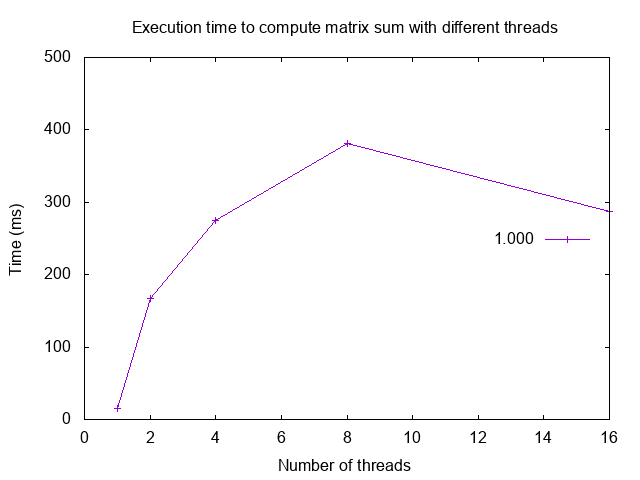
\includegraphics[scale=0.5]{Matrix - 1k.png}
\caption{Benchmarking of matrix computation with 1.000 elements}
\end{figure}      

\clearpage

\begin{verbatim}
5.000 elements

1   387.737	   
2   3725.93     0,104
4   6809.2      0,056    
8   9500.23     0,040   
16  6594.98     0,058   
\end{verbatim}

\begin{figure}[h]
\centering
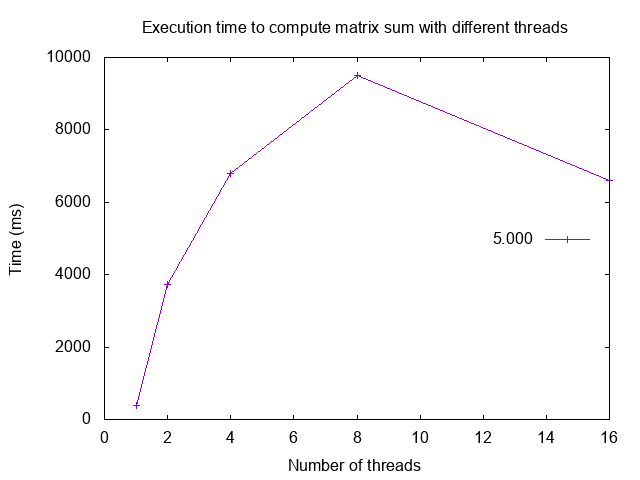
\includegraphics[scale=0.5]{5k.png}
\caption{Benchmarking of matrix computation with 5.000 elements}
\end{figure}      
\clearpage

\begin{verbatim}

10.000 elements

1   1370.3   
2   692.843     1,978
4   346.72      3,952   
8   173.926     7,878  
16  173.945     7,877
\end{verbatim}
\begin{figure}[h]
\centering
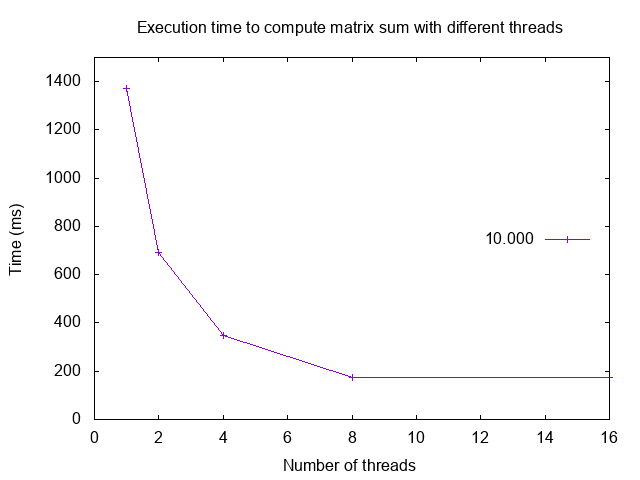
\includegraphics[scale=0.5]{Matrix - 10k.png}
\caption{Benchmarking of matrix computation with 10.000 elements}
\end{figure}      
\clearpage
\begin{verbatim}
100.000 elements

1   12335.1		       
2   6220.19     1,983       
4   3118.69     3,955      
8   1560.34     7,905       
16  1605.09     7,685      
\end{verbatim}

\begin{figure}[h]
\centering
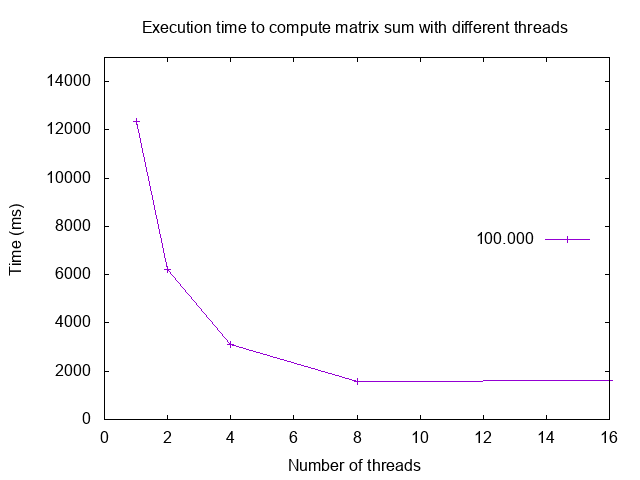
\includegraphics[scale=0.5]{Matrix - 100k.png}
\caption{Benchmarking of matrix computation with 100.000 elements}
\end{figure}      
\clearpage


\subsection{Parallel Quicksort}

\begin{verbatim}

Threads     Execution time (ms)     Speedup

1.000 elements

1   2.168692			
2   2.251632        0,963
4   2.321036        0,934		
8   2.507466        0,865 
16  2.748051        0,789
\end{verbatim}

\begin{figure}[h]
\centering
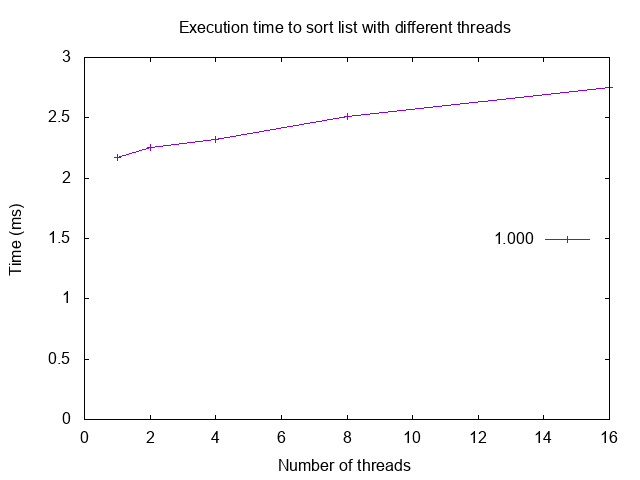
\includegraphics[scale=0.5]{Quicksort - 1k.png}
\caption{Benchmarking of Quicksort 1.000 elements}
\end{figure}      
\clearpage

\begin{verbatim}
    
10.000 elements

1   15.793323 
2   7.663426        2,060 
4   5.406020        2,921	 
8   2.973309        5,311 
16  3.316422        4,762

\end{verbatim}

\begin{figure}[h]
\centering
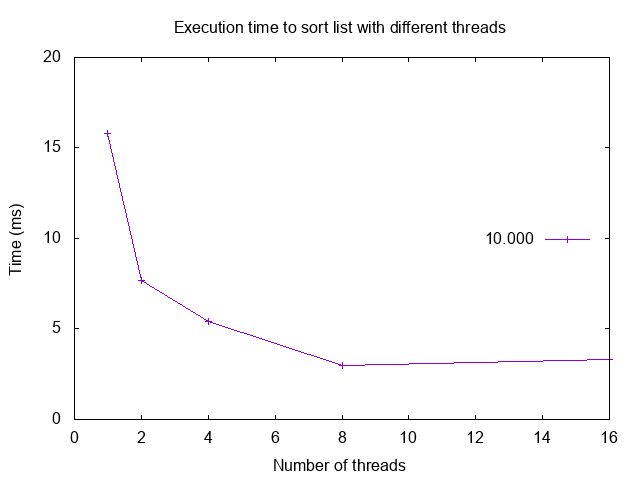
\includegraphics[scale=0.5]{Quicksort - 10k.png}
\caption{Benchmarking of Quicksort 10.000 elements}
\end{figure}      
\clearpage


\begin{verbatim}
    

50.000 elements

1   81.418417	 
2   39.824303       2,044  
4   20.944908       3,887	 
8   11.978569       6,797	 
16  7.685462        10,594 
 
\end{verbatim}

\begin{figure}[h]
\centering
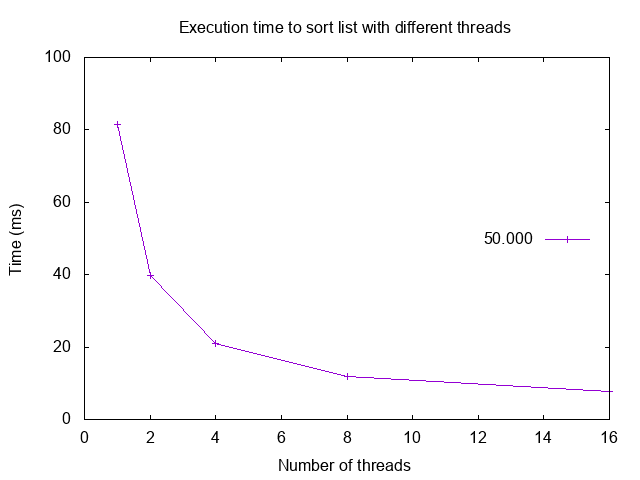
\includegraphics[scale=0.5]{Quiccksort - 50k.png}
\caption{Benchmarking of Quicksort 50.000 elements}
\end{figure}      
\clearpage


\begin{verbatim}
 
100.000 elements

1   152.447315
2   75.687448       2,014
4   37.050616       4,114
8   21.121914       7,217	
16  13.331709       11,434

\end{verbatim}

\begin{figure}[h]
\centering
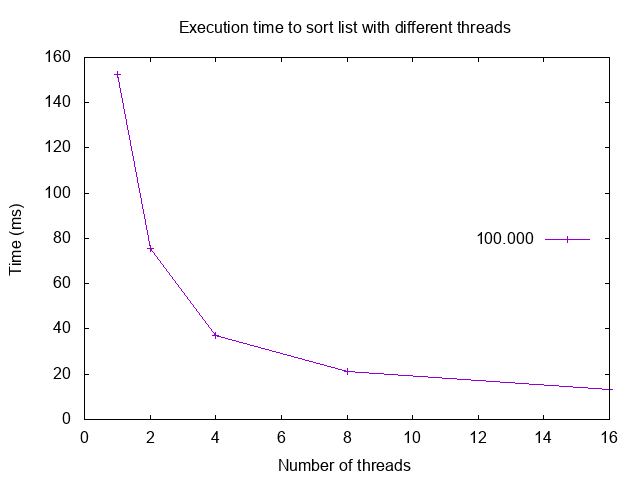
\includegraphics[scale=0.5]{Quicksort - 100k.png}
\caption{Benchmarking of Quicksort 100.000 elements}
\end{figure}      
\clearpage

\subsection{Find palindromic words }

\begin{verbatim}

Threads     Execution time (ms)     Speedup

File with 25.143 words

1   15.716
2   10.110      1,554
4   6.26        2,509
8   4.864       3,231 
16  5.887       2,667
\end{verbatim}

\begin{figure}[h]
\centering
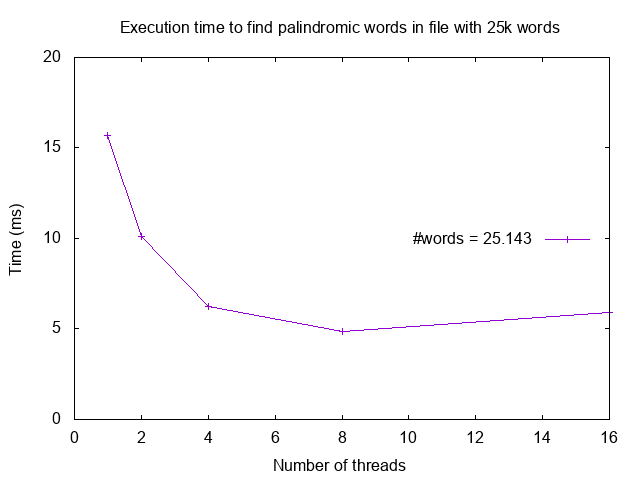
\includegraphics[scale=0.5]{words.png}
\caption{Benchmarking of searching for palindromic words}
\end{figure}      
\clearpage

\begin{verbatim}
    
File with 370.102 words 

1   333.808		
2   215.434     1,5460
4   128.064     2,606
8   80.746      4,134
16  68.294      4,887

\end{verbatim}

\begin{figure}[h]
\centering
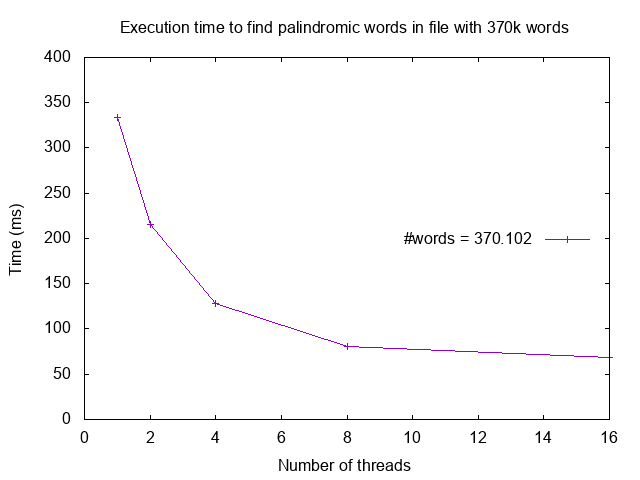
\includegraphics[scale=0.5]{words-alpha.png}
\caption{Benchmarking of searching for palindromic words}
\end{figure}      

\section{Conclusions}

The result shows that at small data-sets the execution times are worse when utilizing multiple threads. This is most probably due to overhead cost of creating threads. However, when the number of elements gets over approximately 10.000 the results shows a clear improvement in execution time when utilizing multiple threads. When the data-sets gets reasonably big the overhead cost gets negligible. 


\end{document}
